\chapter{Falling Bodies}

Gravity exists all around us. If you throw a hammer straight up in the air, from
the moment it leaves your hand until it hits the ground, it is
accelerating toward the center of the earth at a constant rate.

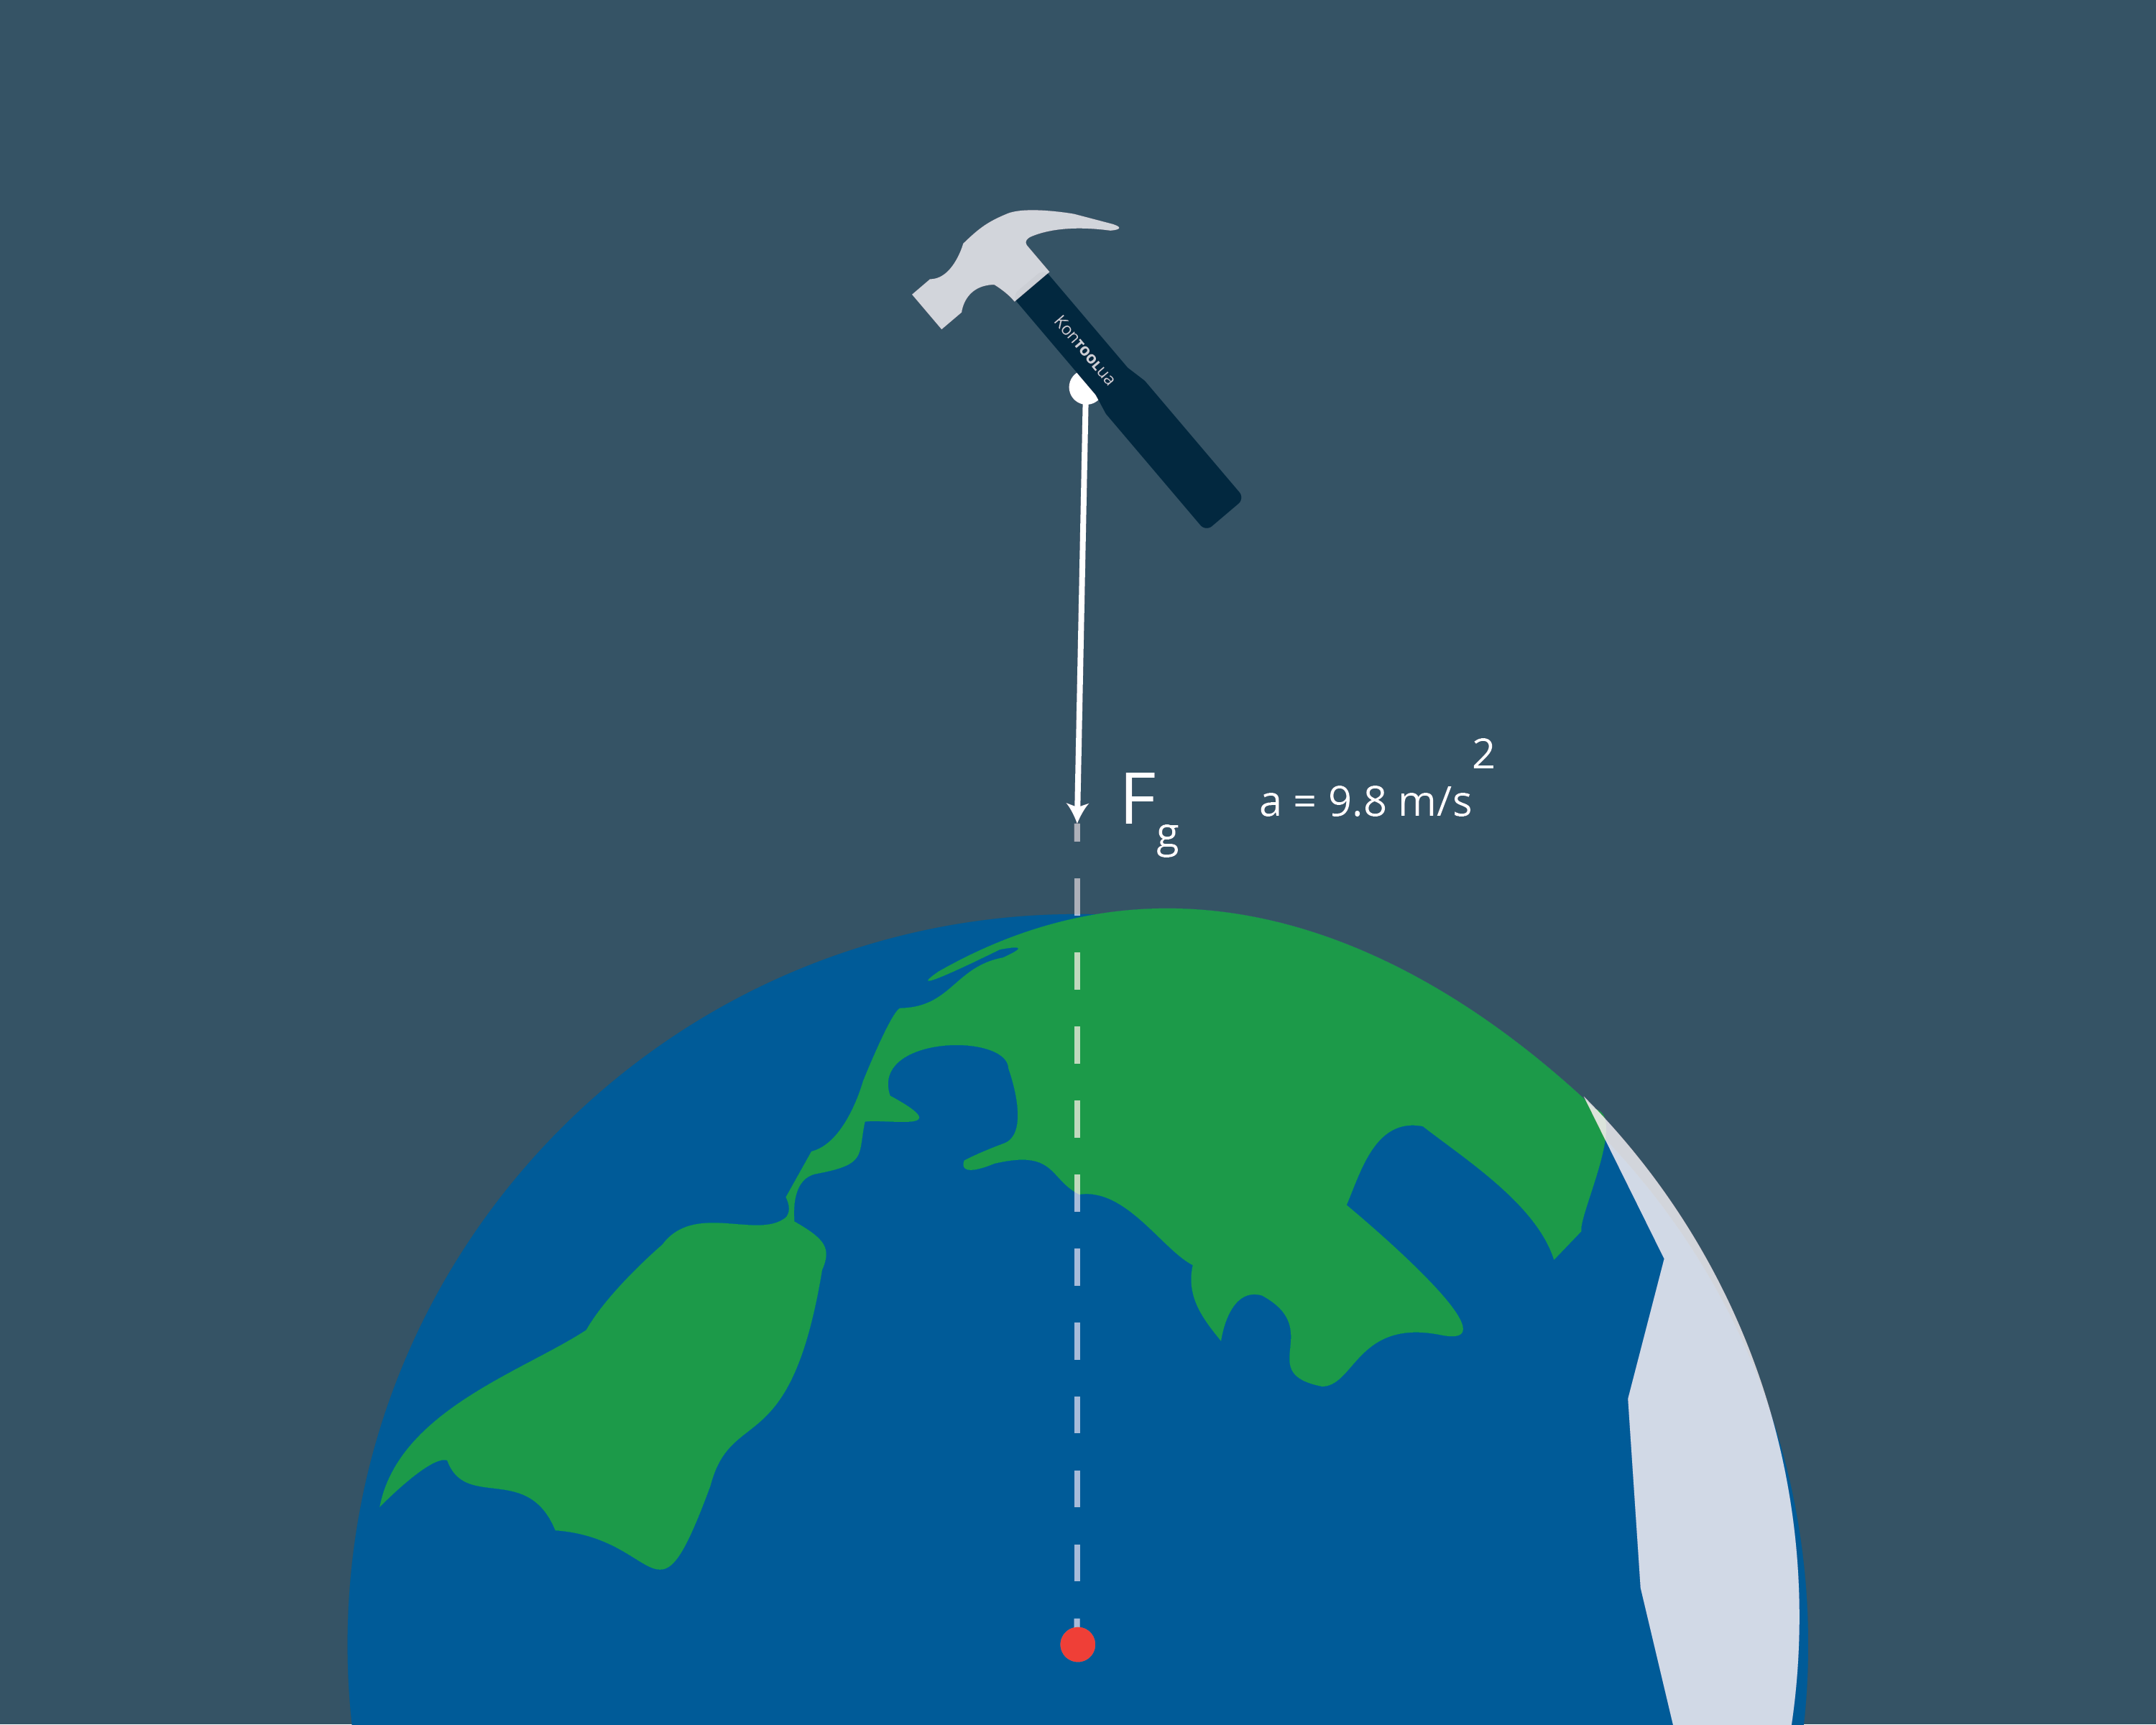
\includegraphics[width=1\textwidth]{hammerFall.png}

\emph{Acceleration} can be defined as change in velocity. If the hammer leaves your
hand with a velocity of 12 meters per second upward, one second later,
it will be rising, and its velocity will have slowed to 2.2 meters per
second. One second after that, the hammer will be falling at a rate of
7.6 meters per second. Every second the hammer's velocity is changing by
9.8 meters per second, and that change is always toward the center of
the earth. When the hammer is going up, gravity is slowing it down by
9.8 meters per second, each second it is in the air.  When the hammer is coming down,
gravity is increasing the speed of its descent by 9.8 meters per second.\index{acceleration}
% Connect to vectors
%right now vectors is after falling bodies, suggest we hint at vectors and in vectors recall this to give students something familiar to anchor them when vectors are introduced


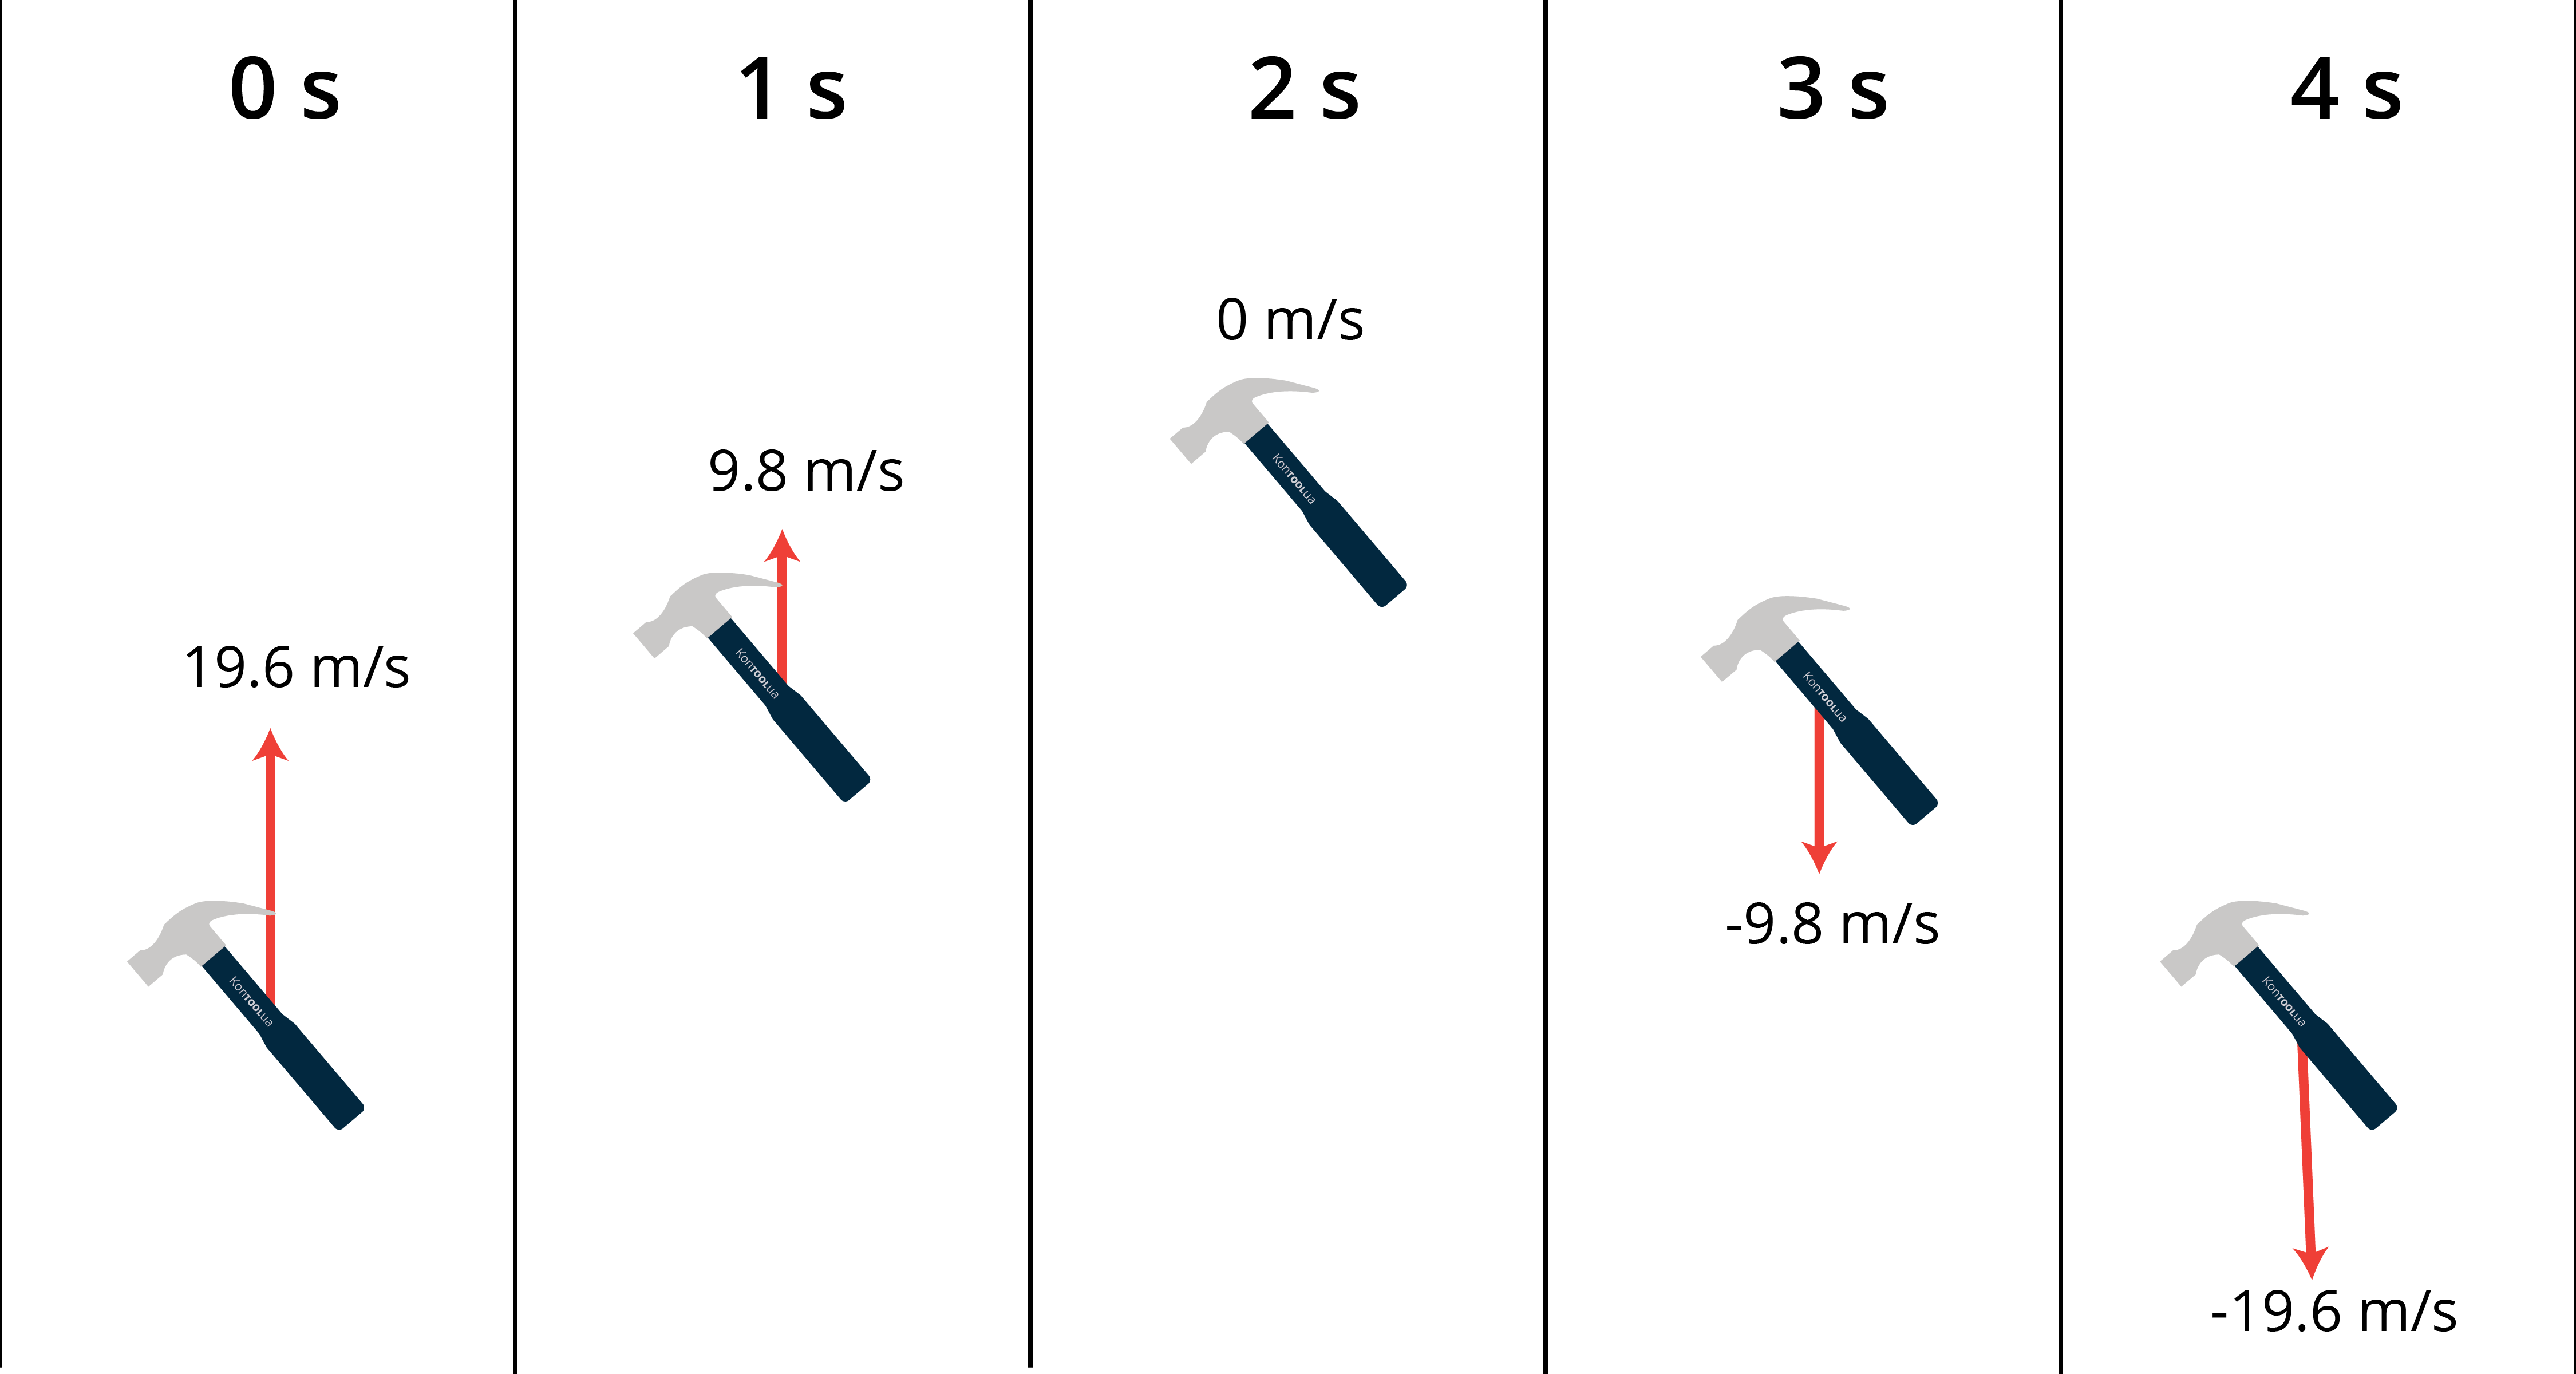
\includegraphics[width=.8\textwidth]{hammerTime.png}

Acceleration due to gravity on earth is a constant negative 9.8 meters per second per second:
\begin{equation*}
a = -9.8 \frac{m}{s^2}  
\end{equation*}
(Why is it negative? We are talking about height, which is generally considered to be increasing as
you go away from the center of the earth. Since ``up" is the positive direction, we take ``down" as a negative direction. Therefore, since gravity pulls things ``down", the acceleration due to gravity is considered negative.)

\section{Calculating the Velocity}

Given that the acceleration is constant, it makes sense that the
velocity is a straight line. Assuming once again that the hammer
leaves your hand at 12 meters per second, let's create a quick data table and 
graph of the hammer's velocity. Every second, we will subtract 9.8 m/s from the 
previous velocity. 

\begin{center}
\begin{tabular}{|c|c|}\hline
Time elapsed (s) & Velocity (m/s)\\\hline
0 & 12\\\hline
1 & 2.2\\\hline
2 & -7.6\\\hline
\end{tabular}
\end{center}

Here is a plot of these data with a dashed fit line:
\begin{center}
\begin{tikzpicture}
\draw[thick, black, latex-latex] (-0.5, 0) -- (6.5, 0) node[below] {$t(s)$};
\draw[thick, black, latex-latex] (0, -3.5) -- (0, 3.5) node[left] {$v(m/s)$};
\draw[] (2, -0.15) -- (2, 0.15) node[below, yshift=-0.35cm] {1};
\draw[] (4, -0.15) -- (4, 0.15) node[below, yshift=-0.35cm] {2};
\draw[] (6, -0.15) -- (6, 0.15) node[below, yshift=-0.35cm] {3};
\draw[] (0.15, 1) -- (-0.15, 1) node[left] {4};
\draw[] (0.15, 2) -- (-0.15, 2) node[left] {8};
\draw[] (0.15, 3) -- (-0.15, 3) node[left] {12};
\draw[] (0.15, -1) -- (-0.15, -1) node[left] {-4};
\draw[] (0.15, -2) -- (-0.15, -2) node[left] {-8};
\draw[] (0.15, -3) -- (-0.15, -3) node[left] {-12};

\draw[black, fill=black] (0, 3) circle (0.075cm);
\draw[black, fill=black] (2, 0.55) circle (0.075cm);
\draw[black, fill=black] (4, -1.9) circle (0.075cm);
\draw[thin, dashed] (0, 3) -- (4.9, -3);
\end{tikzpicture}
\end{center}

We can find an equation for the line: $v = 12 - 9.8t$. What is this saying? It 
says that at any time, $t$, after $t=0s$, the velocity of the hammer is its 
starting velocity (12 m/s) plus the acceleration (-9.8 m/s$^2$) multiplied by 
the time elapsed ($t$). (Why did we say ``plus" instead of ``minus"? Well, 
since the acceleration \textit{is negative}, $v_0-9.8t$ is the same as $v_0 + 
\left( -9.8t \right)$, and we are really adding the negative acceleration. When 
the acceleration is positive, we'll see a plus sign!)

\begin{Exercise}[title={When is the apex of flight?}, label=vapex]
  Given the hammer's velocity is calculated as $12 - 9.8t$, at what time (in 
  seconds) does it stop rising and begin to fall?
\end{Exercise}
\begin{Answer}[ref=vapex]
  At it's apex, the hammer's velocity is $0 m/s$, so we will find the time 
  where $v=0m/s$:
  $$0 \frac{m}{s} = 12 \frac{m}{s} - 9.8 \frac{m}{s^2} \cdot t$$
  $$t = \frac{12 \frac{m}{s}}{9.8 \frac{m}{s^2}} \approx 1.22s$$
\end{Answer}

We can generalize this to other falling bodies. For any falling object with 
initial velocity  $v_0$ and constant acceleration $a$, its velocity is given 
by:
$$v(t) = v_0 + a \cdot t$$

\textbf{Example}: The acceleration due to gravity on the Moon is approximately 
1.63 m/s$^2$. If a hammer tossed upwards on the Moon takes 3.4 seconds to reach 
its apex, what was the hammer's initial velocity?

\textbf{Solution}: We know that $a = -1.63 m/s^2$ and $t = 3.4s$. Substituting 
and solving the velocity equation:
$$0 \frac{m}{s} = v_0 + \left( -1.63 \frac{m}{s^2} \right) \left( 3.4 s \right)$$
$$v-0 = \left( 1.63 \cdot 3.4 \right) \frac{m}{s} \approx 5.5 \frac{m}{s}$$

This hammer must have been tossed upwards with an initial velocity of 
approximately 5.5 m/s.

\subsection{Air Resistance}

At this point, we need to acknowledge air resistance. Gravity
is not the only force on the hammer; as it travels through the air,
friction with the air slows it down. This force is called \emph{air resistance},
and for a large, fast-moving object (like an airplane) it is GIGANTIC force. 
For a dense object (like a hammer) moving at a slow speed (what you generate
with your hand), air resistance doesn't significantly affect acceleration.

Consider two otherwise identical pieces of paper: one completely flat and 
unfolded, the other balled up as tightly as possible. If you dropped them both 
from the same height, which would hit the ground first? Intuitively, you know 
the balled-up paper would: but \textit{why}? Since the papers have the same 
mass, you know that the force of gravity is the same on both papers! However, 
if you give this a try (go ahead, all you need to two sheets of printer paper 
and a safe place to drop them from), the acceleration of the two papers is 
different. 

We can apply Newton's Second Law to explain our observations. First, let's draw 
diagrams to represent the forces acting on the papers:

\begin{center}
    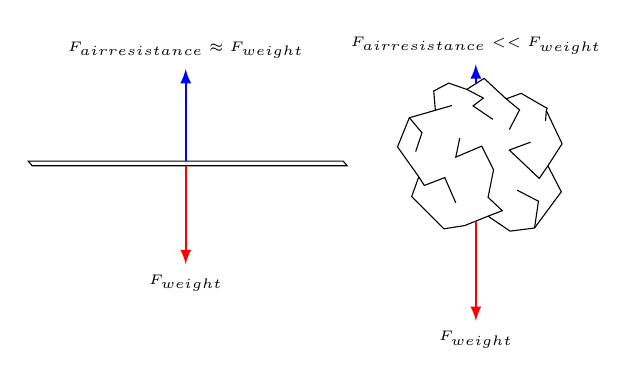
\begin{tikzpicture}
        %crumpled paper
        \draw[] (1.02, 1.94) -- (1.24, 2.08) --(1.52, 1.82) -- (1.69, 1.68) -- 
        (1.56, 1.43);
        \draw[] (1.52, 1.82) -- (1.71, 1.89) -- (2.04, 1.7) -- (2.03, 1.67) -- 
        (2.02, 1.54);
        \draw[] (2.03, 1.67) -- (2.23, 1.25) -- (2.05, 0.97) -- (1.94, 0.81) -- 
        (1.56, 1.17) -- (1.83, 1.27);
        \draw[] (2.05, 0.97) -- (2.22, 0.64) -- (1.88, 0.18) -- (1.57, 0.14) -- 
        (1.29, 0.33);
        \draw[] (1.88, 0.18) -- (1.93, 0.52) -- (1.66, 0.66);
        \draw[] (0.93, 1.32) -- (0.88, 1.08) -- (1.21, 1.22) -- (1.36, 0.92) -- 
        (1.29, 0.57) -- (1.47, 0.4) -- (1.29, 0.33) -- (0.99, 0.21) -- 
        (0.73, 0.17) -- (0.32, 0.58) -- (0.41, 0.83);
        \draw[] (0.88, 0.5) -- (0.74, 0.82) -- (0.48, 0.72) -- (0.41, 0.83) -- 
        (0.14, 1.21) -- (0.29, 1.58) -- (0.83, 1.735);
        \draw[] (0.37, 1.15) -- (0.45, 1.39) -- (0.29, 1.58);
        \draw[] (0.62, 1.68) -- (0.6, 1.92) -- (0.79, 2.02) -- (1.02, 1.94) -- 
        (1.23, 1.83) -- (1.1, 1.73) -- (1.35, 1.56);
        \draw[blue, thick, -latex] (1.135, 2.01) -- (1.135, 2.26) 
        node[above, black, font = \tiny] {$F_{\text{air resistance}} << 
        F_{\text{weight}}$};
        \draw[red, thick, -latex] (1.135, 0.27) -- (1.135, -1) 
        node[below, black, font = \tiny] {$F_{\text{weight}}$};

        %flat paper
        \draw[] (-0.55, 1.03) -- (-4.55, 1.03) -- (-4.5, 0.97) -- (-0.5, 0.97) 
        -- cycle;
        \draw[blue, thick, -latex] (-2.55, 1.03) -- (-2.55, 2.2) 
        node[above, black, font = \tiny] {$F_{\text{air resistance}} \approx 
        F_{\text{weight}}$};
        \draw[red, thick, -latex] (-2.55, 0.97) -- (-2.55, -0.28) 
        node[below, black, font = \tiny] {$F_{\text{weight}}$};
        \end{tikzpicture}
\end{center}

For the crumpled paper, the decrease in surface area results in very little air 
resistance. As a result, the net force on the crumpled paper is approximately 
equal to the paper's weight. 
$$F_{\text{net}}^{\text{crumpled}} = F_{\text{air resistance}} + 
F_{\text{weight}} \approx F_{\text{weight}}$$
$$F_{\text{net}}^{\text{crumpled}} = ma_{\text{crumpled}} \approx 
F_{\text{weight}} = mg$$
$$a_{\text{crumpled}} \approx g$$

Thus, you observe the crumpled paper to fall at nearly -9.8 m/s$^2$. The flat 
paper, on the other hand, has a much larger surface area, and therefore 
experiences significantly more air resistance. Thus, the observed acceleration 
of the flat paper is much slower:
$$F_{\text{net}}^{\text{flat}} = F_{\text{air resistance}} + 
F_{\text{weight}}$$
$$ma_{\text{flat}} = F_{\text{air resistance}} + mg$$
$$a_{\text{flat}} = \frac{F_{\text{air resistance}}}{m} + g$$

Since $g<0$ and $F_{\text{air resistance}}$ is positive, the greater the air 
resistance the slower the paper falls. 
% Relate to f=ma
%here's an F=ma example for air resistance that students can observe at home

\section{Calculating Position}

If you let go of the hammer when it is 2 meters
above the ground, the height of the hammer is given by:
\begin{equation*}
  p = -\frac{9.8}{2}t^2 + 12t + 2
\end{equation*}

Here is a graph of this function:

\begin{tikzpicture}
    \begin{axis}[
        xmin=-1.2,xmax=3.5,
        ymin=-13,ymax=13,
        axis x line=middle,
        axis y line=middle,
        axis line style=<->,
        xlabel={$t$},
        ylabel={$p$},
      ]
      \addplot[no marks,sdkblue,dashed,<-] expression [domain=-0.7:0,samples=100] 
      {(-4.9)*(x^2) + 12 * x + 2};
      \addplot[no marks,sdkblue] expression [domain=0:2.58,samples=100] 
      {(-4.9)*(x^2) + 12 * x + 2};
      \addplot[no marks,sdkblue,dashed,->] expression [domain=2.58:3,samples=100] 
      {(-4.9)*(x^2) + 12 * x + 2};
    \end{axis}
\end{tikzpicture}


How do we know? \textbf{The change in position between time
  $0$ and any time $t$ is equal to the area under the velocity graph
  between $x = 0$ and $x = t$.}

Let's use the velocity graph to figure out how much the position has
changed in the first second of the hammer's flight. Here is the
velocity graph with the area under the graph for the first second filled
in:

\usepgfplotslibrary{fillbetween}

\begin{tikzpicture}
    \begin{axis}[
        xmin=-0.25,xmax=2.75,
        ymin=-13,ymax=13,
        axis x line=middle,
        axis y line=middle,
        axis line style=<->,
        xlabel={$t$},
        ylabel={$v$},
      ]
      \addplot[no marks,sdkblue, name path=f] 
      	expression[domain=0:2.25,samples=100]
      	{x * (-9.8) + 12} node[left] {$12 - 9.8t$};
      \path[name path=xaxis] (axis cs:0,0) -- (axis cs:1,0);
      \addplot[
        thick,
        color=sdkblue,
        fill=sdkblue, 
        fill opacity=0.05
    ]
    fill between[
        of=f and xaxis,
        soft clip={domain=0:1},
    ];
    \addplot[dashed,gray] coordinates {(0,12)(1,12)};
    \addplot[dashed,gray] coordinates {(1,12)(1,0)};
    \end{axis}
\end{tikzpicture}

The blue filled region is the area of the dashed rectangle minus that
empty triangle in its upper left.  The height of the rectangle is
twelve and its width is the amount of time the hammer has been in
flight ($t$). The triangle is $t$ wide and $9.8t$ tall. Thus, the
area of the blue region is given by $12t - \frac{1}{2}9.8 t^2$.

That's the change in position. Where was it originally? 2 meters off
the ground. This means the height is given by $p = 2 + 12t - \frac{1}{2}9.8t^2$.
We usually write terms so that the exponent decreases, so:

$$p = - \frac{1}{2}9.8t^2 + 12t + 2$$

Finding the area under the curve like this is called
\textit{integration}. We say ``To find a function that gives the
change in position, we just integrate the velocity function.''  Much
of the study of calculus is learning to integrate different sorts of
functions.\index{integration}

One important note about integration: Any time the curve drops under
the $x$-axis, the area is considered negative. (Which makes sense,
right? If the velocity is negative, the hammer's position is
decreasing.)


\begin{tikzpicture}
    \begin{axis}[
        xmin=-0.25,xmax=2.75,
        ymin=-13,ymax=13,
        axis x line=middle,
        axis y line=middle,
        axis line style=<->,
        xlabel={$t$},
        ylabel={$v$},
      ]
      \addplot[no marks,sdkblue, name path=f] 
      expression[domain=0:2.25,samples=100]
      {x * (-9.8) + 12} node[left] {$12 - 9.8t$};
      \path[name path=xaxis] (axis cs:0,0) -- (axis cs:2.25,0);
      \addplot[
        thick,
        color=sdkblue,
        fill=sdkblue, 
        fill opacity=0.05
      ]
      fill between[
        of=f and xaxis,
        soft clip={domain=0:1.2245},
      ];
      \addplot[
        thick,
        color=red,
        fill=red, 
        fill opacity=0.07
      ]
      fill between[
        of=f and xaxis,
        soft clip={domain=1.2245:2.1},
      ];
    \end{axis}
\end{tikzpicture}


\section{Quadratic functions}

Functions of the form $f(x) = a x^2 + b x + c$ are called 
\newterm{quadratic functions}. 
If $a > 0$, the ends go up.
If $a < 0$, the ends go down.\index{quadratic functions}


\begin{tikzpicture}
  \begin{axis}[
      xmin=-2.2,xmax=1.2,
      ymin=-2,ymax=3,
      axis x line=middle,
      axis y line=middle,
      axis line style=<->,
    ]
    \addplot[no marks,sdkblue] expression [domain=-2:1,samples=100] 
    	{(2)*(x^2) + 2 * x - 1};
  \end{axis}
  \node[right] at (1,4) {$2x^2 + 2x - 1$};
\end{tikzpicture}
\hspace{4mm}
\begin{tikzpicture}
  \begin{axis}[
    xmin=-1.5,xmax=1.5,
    ymin=-2,ymax=1.5,
    axis x line=middle,
    axis y line=middle,
    axis line style=<->,
  ]
  \addplot[no marks,sdkblue] 
  	expression [domain=-1.5:1.5,samples=100] 
  	{(-1.2)*(x^2) + 0.5 * x + 1};
\end{axis}
\node[right] at (0.5,1) {$-1.2 x^2 + 0.5 x + 1$};
\end{tikzpicture}

The graph of a quadratic function is a \newterm{parabola}.

\section{Simulating a falling body in Python}

Now you are going to write some Python code that simulates the flying hammer. 
First, we are just going to print out the position, speed, and acceleration of 
the hammer for every 1/100th of a second after it leaves your hand. (Later, we 
will make a graph.)

Create a file called \filename{falling.py} and type this into it:

\begin{Verbatim}
# Acceleration on earth
acceleration = -9.8 # m/s/s

# Size of time step
time_step = 0.01 # seconds

# Initial values
speed = 12  # m/s upward
height = 2  # m above the ground
current_time = 0.0  # seconds after release

# Is the hammer still aloft?
while height > 0.0:

    # Show the values
    print(f"{current_time:.2f} s:")
    print(f"\tacceleration: {acceleration:.2f} m/s/s")
    print(f"\tspeed: {speed:.2f} m/s")
    print(f"\theight: {height:.2f} m")

    # Update height
    height = height + time_step * speed

    # Update speed
    speed = speed + time_step * acceleration

    # Update time
    current_time = current_time + time_step


print(f"Hit the ground: Complete")
\end{Verbatim}

When you run it, you will see something like this:
\begin{Verbatim}
0.00 s:
	acceleration: -9.80 m/s/s
	speed: 12.00 m/s
	height: 2.00 m
0.01 s:
	acceleration: -9.80 m/s/s
	speed: 11.90 m/s
	height: 2.12 m
0.02 s:
	acceleration: -9.80 m/s/s
	speed: 11.80 m/s
	height: 2.24 m
0.03 s:
	acceleration: -9.80 m/s/s
	speed: 11.71 m/s
	height: 2.36 m
...
2.60 s:
	acceleration: -9.80 m/s/s
	speed: -13.48 m/s
	height: 0.20 m
2.61 s:
	acceleration: -9.80 m/s/s
	speed: -13.58 m/s
	height: 0.07 m
Hit the ground: Complete
\end{Verbatim}

Note that the acceleration isn't changing at all, but it is changing
the speed, and the speed is changing the height.

We can see that the hammer in our simulation hits the ground just
after 2.61 seconds.

\subsection{Graphs and Lists}

Now, we are going to graph the acceleration, speed, and height using a
library called matplotlib. However, to make the graphs, we
need to gather all the data into lists.\index{matplotlib}

For example, we will have a list of speeds, and the first three
entries will be 12.0, 11.9, and 11.8.\index{lists, python}

We create an empty list and assign it to a variable like this:
\begin{Verbatim}
x = []
\end{Verbatim}

Next, we can add items like this:
\begin{Verbatim}
x.append(3.14)
\end{Verbatim}

To get the first time back, we can ask for the object at index 0.
\begin{Verbatim}
y = x[0]
\end{Verbatim}
Note that the list starts at 0. If you have 32 items in the list,
the first item is at index 0; the last item is at index 31.

Duplicate the file \filename{falling.py} and name the new copy 
\filename{falling\_graph.py}

We are going to make a plot of the height over time. At the start of the 
program, you will import the matplotlib library.  At the end of the program, 
you will create a plot and show it to the user.

In \filename{falling\_graph.py}, add the bold code:

\begin{Verbatim}[commandchars=\\\{\}]
\textbf{import matplotlib.pyplot as plt}

# Acceleration on earth
acceleration = -9.8 # m/s/s

# Size of time step
time_step = 0.01 # seconds

# Initial values
speed = 12  # m/s upward
height = 2  # m above the ground
current_time = 0.0  # seconds after release

\textbf{# Create empty lists}
\textbf{accelerations = []}
\textbf{speeds = []}
\textbf{heights = []}
\textbf{times = []}

# Is the hammer still aloft?
while height > 0.0:

    \textbf{# Add the data to the lists}
    \textbf{times.append(current_time)}
    \textbf{accelerations.append(acceleration)}
    \textbf{speeds.append(speed)}
    \textbf{heights.append(height)}
    
    # Update height
    height = height + time_step * speed

    # Update speed
    speed = speed + time_step * acceleration

    # Update time
    current_time = current_time + time_step

\textbf{# Make a plot}
\textbf{fig, ax = plt.subplots()}
fig.suptitle("Falling Hammer")
\textbf{ax.set_xlabel("Time (s)")}
\textbf{ax.set_ylabel("Height (m)")}
\textbf{ax.plot(times, heights)}
\textbf{plt.show()}
\end{Verbatim}

When you run the program, you should see a graph of the height over time.

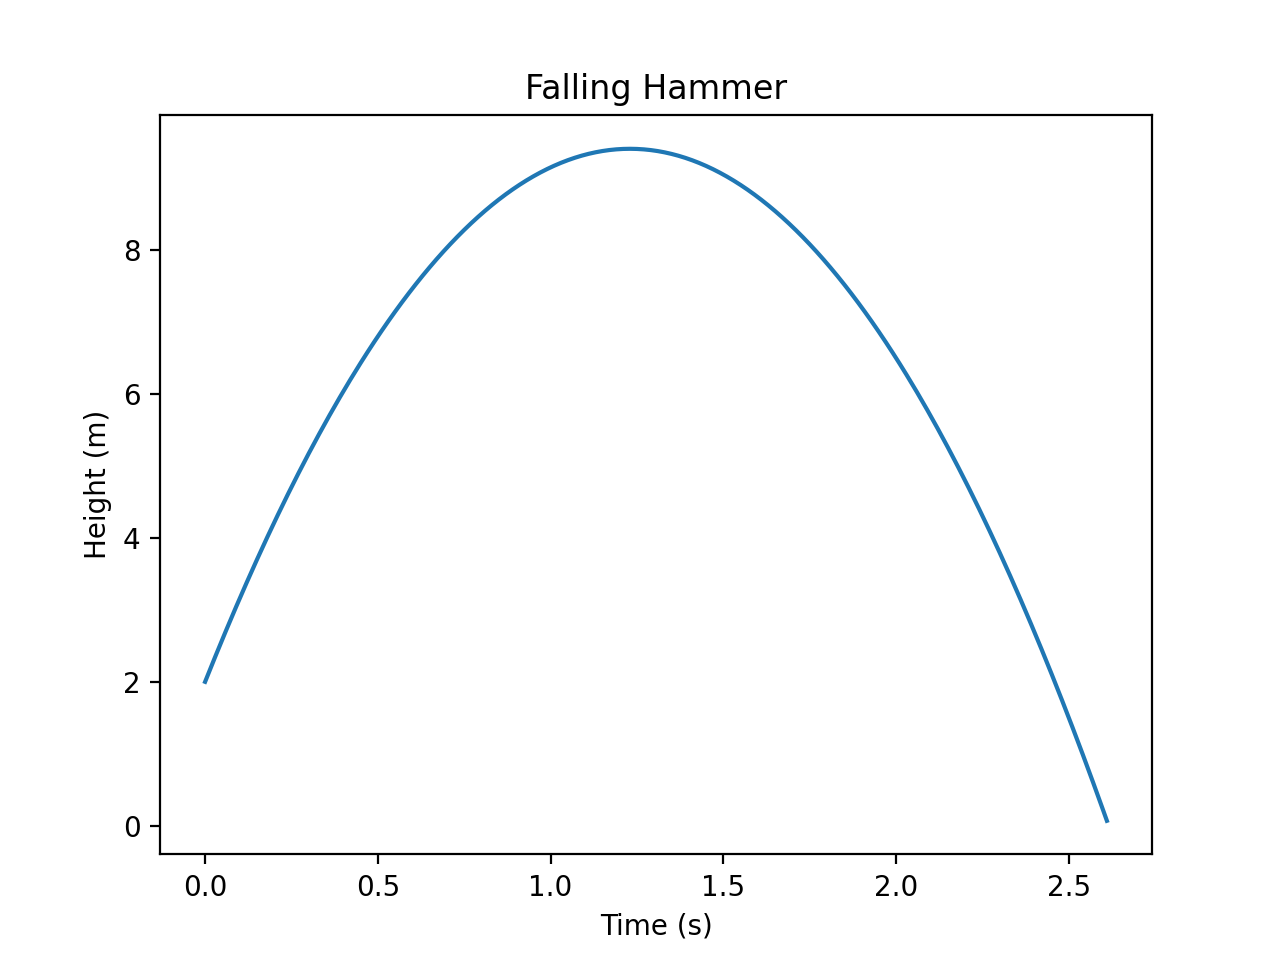
\includegraphics[width=0.7\linewidth]{heightplot.png}

It is more interesting if we can see all three: acceleration, speed, and height. 
So, let's make three stacked plots. Change the plotting code in 
\filename{falling\_graph.py} to:\index{matplotlib!subplots}

\begin{Verbatim}
# Make a plot with three subplots
fig, ax = plt.subplots(3,1)
fig.suptitle("Falling Hammer")

# The first subplot is acceleration
ax[0].set_ylabel("Acceleration (m/s/s)")
ax[0].plot(times, accelerations)

# Second subplot is speed
ax[1].set_ylabel("Speed (m/s)")
ax[1].plot(times, speeds)

# Third subplot is height
ax[2].set_xlabel("Time (s)")
ax[2].set_ylabel("Height (m)")
ax[2].plot(times, heights)
plt.show()
\end{Verbatim}

You will now get plots of all three variables:

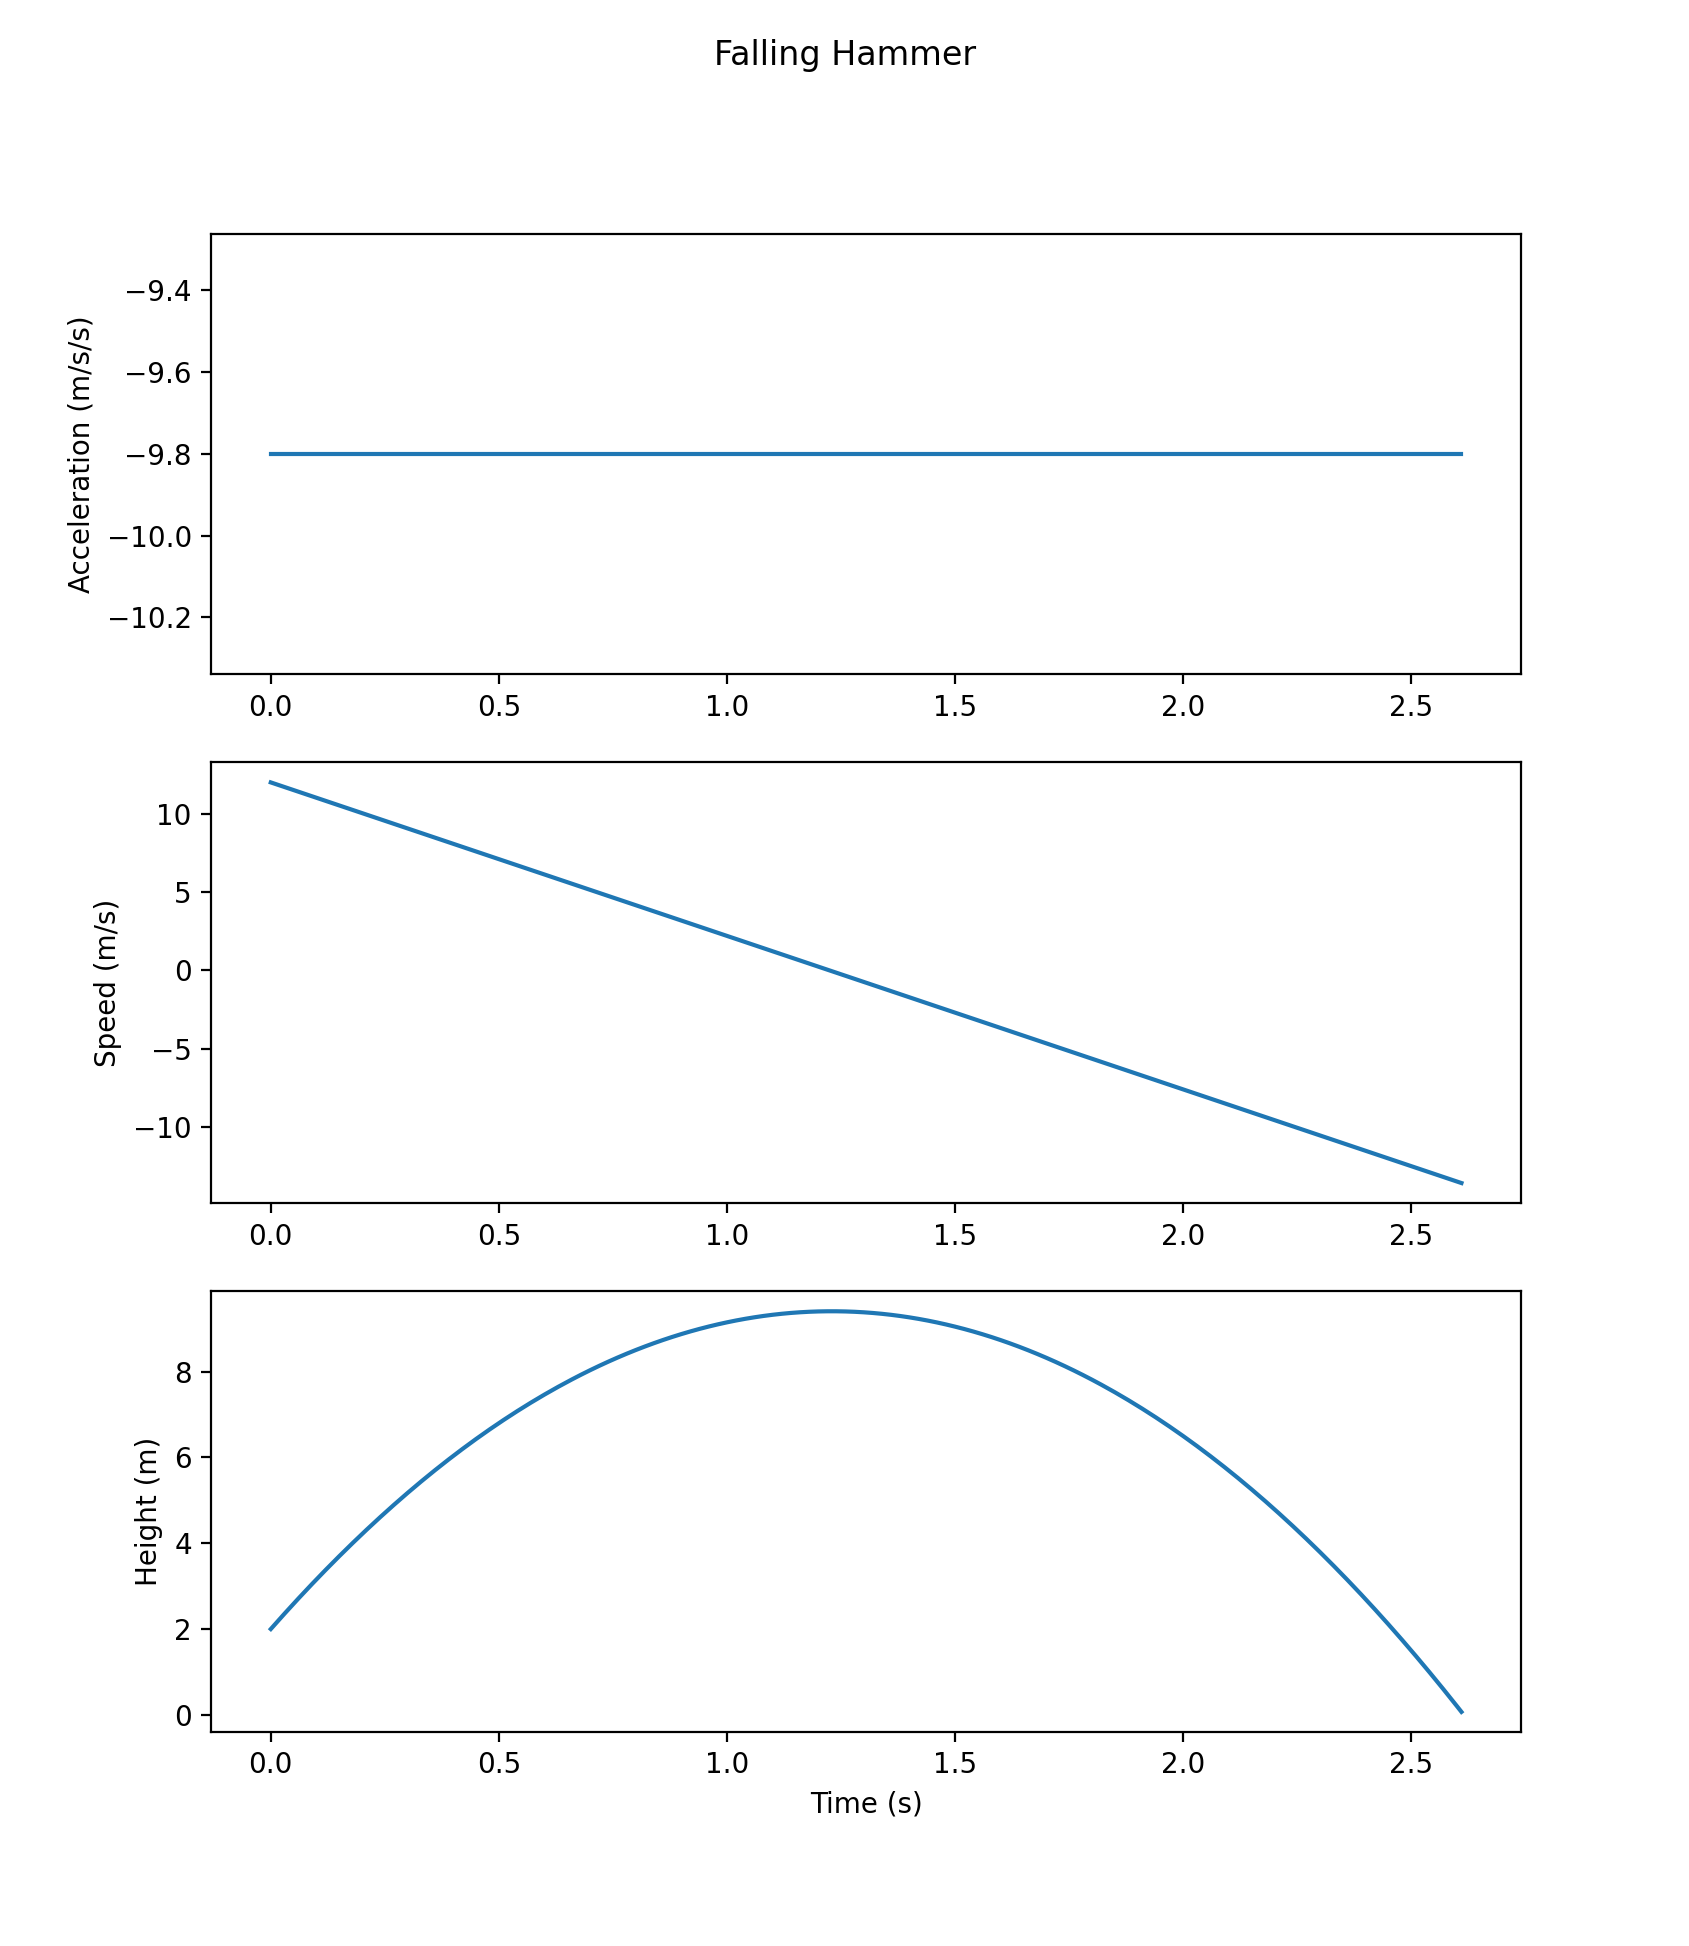
\includegraphics[width=0.8\linewidth]{stackedplot.png}

This is what we expected, right? The acceleration is a constant negative 
number. The speed is a straight line with a negative slope. The height is a 
parabola. \textbf{The slope of the height graph is the speed, and the slope of the speed graph is acceleration}

A natural question at this point is ``When exactly will the hammer hit the
ground?''  In other words, when does $height = 0$? The values of $t$ where a 
function is zero are known as its \textit{roots}. Height is given by a quadratic 
function. In the next chapter, you will get the trick for finding the roots of 
any quadratic function.
